\section{Versuchsdurchführung}
Mit den gefundenen Zusammenhängen aus dem voran gegangenen Abschnitt ist es
möglich das Trägheitsmoment verschiedener Körper experimentell zu bestimmen.
Des Weiteren soll der \textit{Satz von Steiner} \eqref{eq: steiner} überprüft
werden. \\
Der Versuchsaufbau ist in Abbildung (Referenz) dargestellt. Die Körper, deren
Trägheitsmomente bestimmt werden sollen, werden an einer zweifach drehbaren Achse
befestigt. Diese ist über eine Torsionsfeder mit einem raumfesten Rahmen verbunden,
an dem zum Ablesen der Auslenkung aus der Ruhelage eine Winkelskala angebracht ist.

\subsection{Bestimmung der Winkelrichtgröße $D$}
In die Schwingvorrichtung wird horizontal eine Stange eingeschraubt, deren Masse an dieser
Stelle und im Folgenden vernachlässigt werden soll. Eine Federwaage wird im Abstand $a$ zur
Drehachse eingehängt. Durch ziehen an der Federwaage (rechtwinklig zur Stange) wird das System um einen Winkel $\phi$
ausgelenkt. Im Kräftegleichgewicht gilt:
\begin{equation}
  \left| \vec{M} \right| = \left|\vec{r} \times \vec{F} \right| = a \cdot F = D \cdot \phi \iff D = \frac{a \cdot F}{\phi}
\end{equation}
Die Kraftmessung wird für drei Abstände und jeweils vier Auslenkungswinkel durchgeführt.

\subsection{Bestimmung des Eigenträgheitsmomentes $I_D$}
An der Stange werden nun jeweils im Abstand $a$ zur Drehachse zwei Zylinderförmige
Massen $m$ angebracht. Nun wird die Schwingungsdauer mit einer Stoppuhr
aus messpraktischen Gründen für fünf Schwingungen gemessen. Der Abstand $a$ wird zehnmal varriert, wobei jeweils
drei Messungen durchgeführt werden.

\subsection{Messung verschiedener Trägheitsmomente}
Nun soll das Trägheitsmoment eines homogenen Zylinder, einer homogenen Kugel und einer
Malerpuppe gemessen werden. Um den experimentell ermittelten Wert später mit dem theoretischen
vergleichen zu können, werden zunächst die relevanten Größen (siehe Formeln) der Körper
bestimmt. Die Masse mittels einer digitalen Waage, die entsprechenden Längen mit einem
Messchieber. Zylinder und Kugel werden nacheinander auf die Drehvorrichtung geschraubt und
das Zeitintervall für fünf Schwingungen zehn mal gemessen. \\
Die Malerpuppe soll bei der theoretischen Betrachtung durch ein Gebilde aus Körpern mit
bekanntem Trägheitsmoment ersetzt werden. Die entsprechenden Abmessungen und die für den Satz
von Steiner relevanten Abstände zur Rotationsachse werden ebenfalls mit dem Messchieber bestimmt.
Die Puppe wird in zwei verschiedenen Positionen (Abbildung \ref{fig:konfig}) auf die Apperatur aufgebracht
und die Schingungsdauern in gleicher Weise wie bei den anderen Körpern gemessen. \\

\begin{figure}
\centering
\begin{subfigure}{0.48\textwidth}
\centering
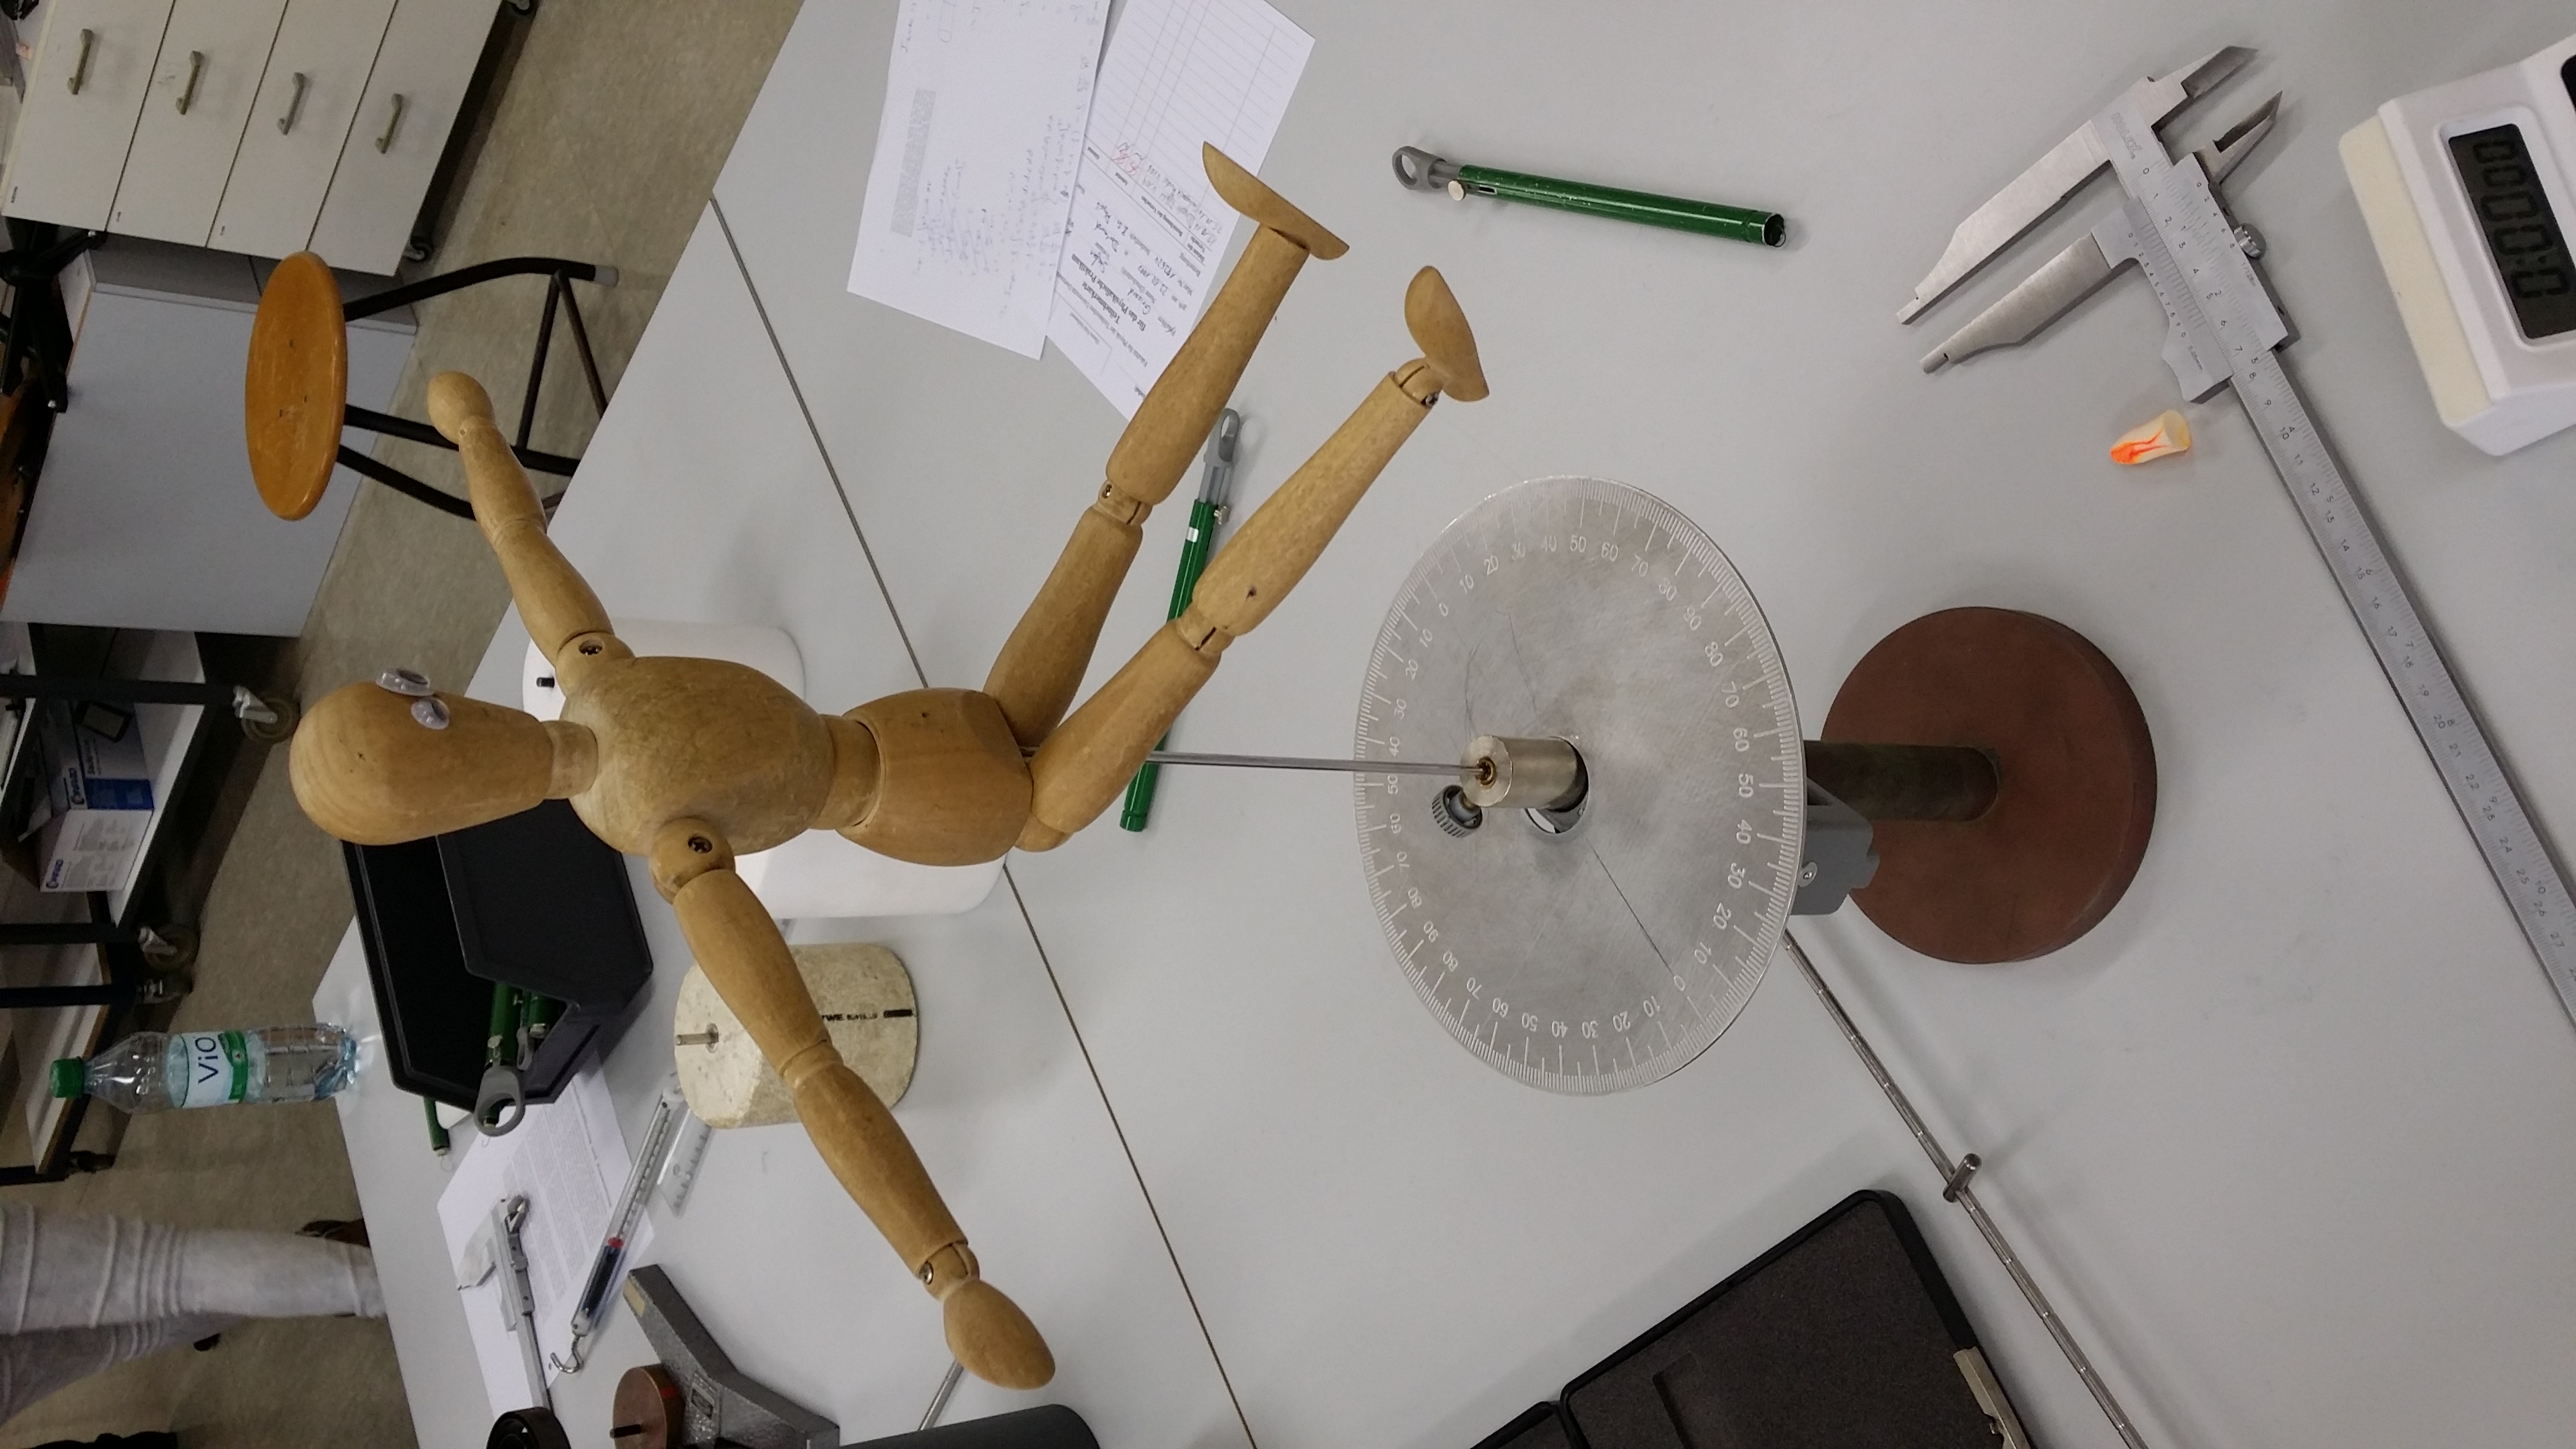
\includegraphics[width = 4cm, angle = 270]{Puppe_1.jpg}
\caption{Position 1}
\label{fig:pup1}
\end{subfigure}
\begin{subfigure}{0.48\textwidth}
\centering
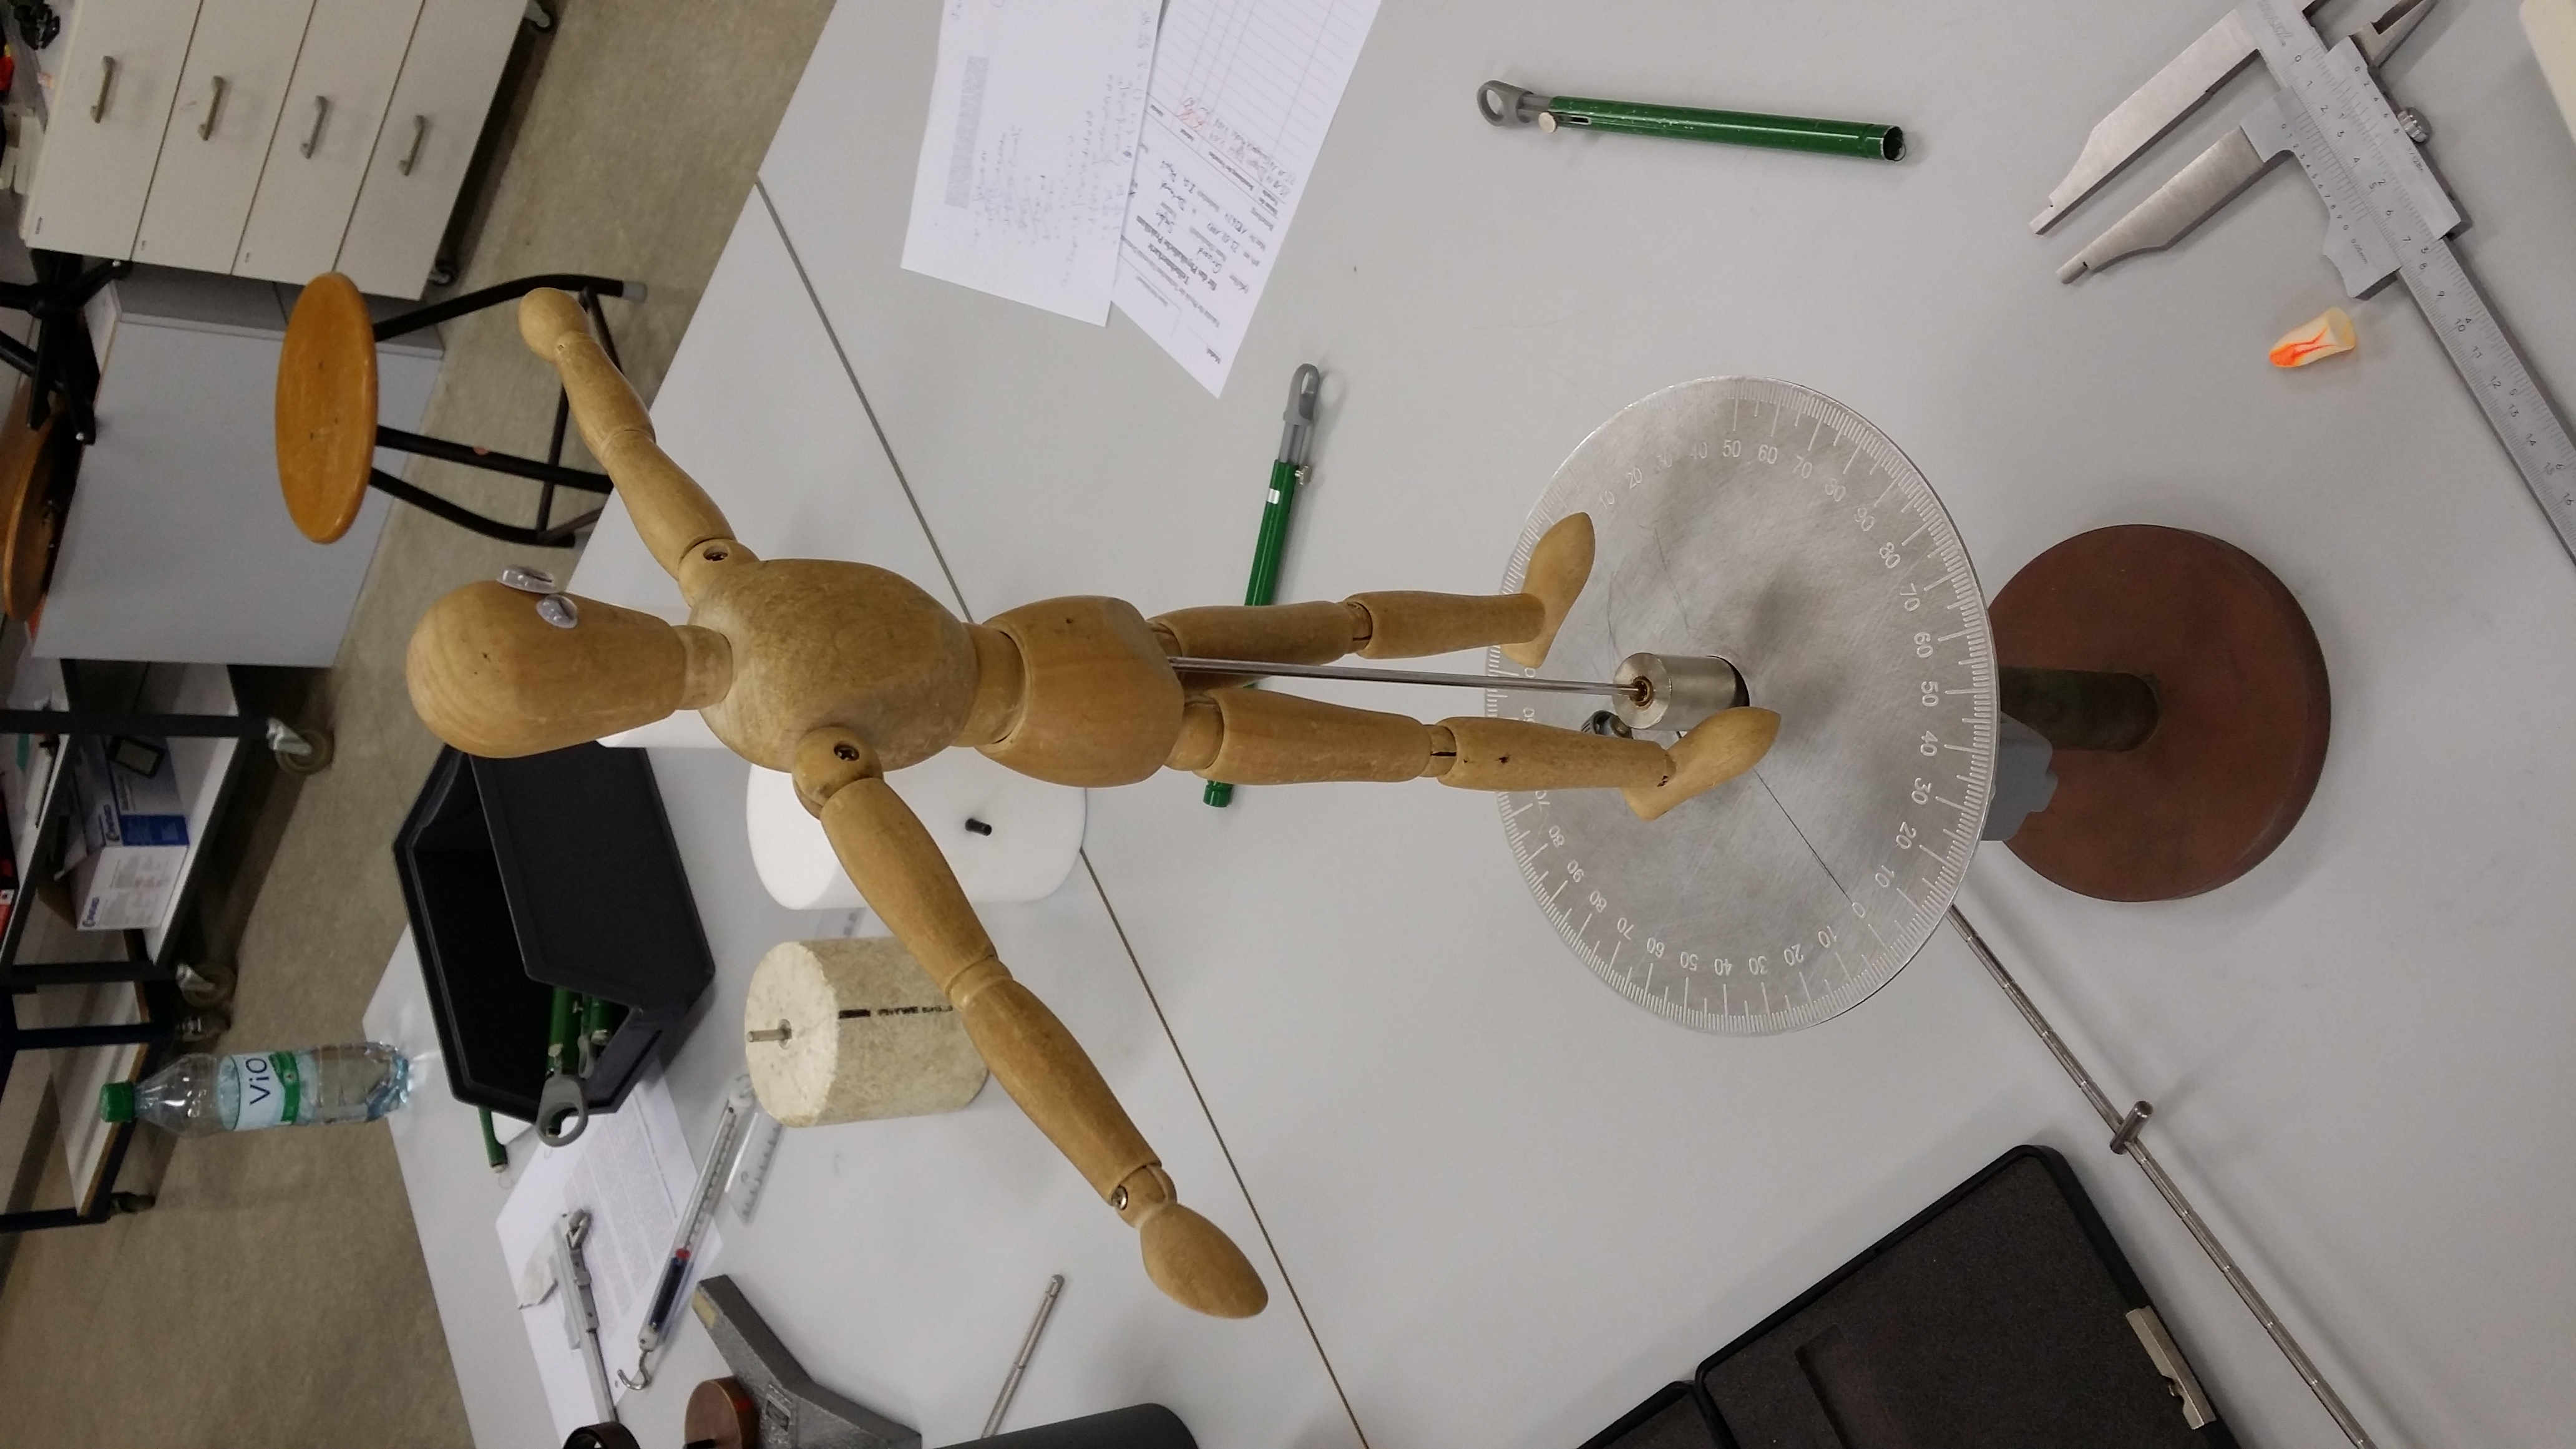
\includegraphics[width=4cm,angle = 270]{Puppe_2.jpg}
\caption{Position 2}
\label{fig:pup2}
\end{subfigure}
\caption{Konfigurationen der Puppe}
\label{fig:konfig}
\end{figure}
